\documentclass[11pt,a4paper]{report}
\usepackage[latin1]{inputenc}
\usepackage[spanish]{babel}
\usepackage{amsmath}
\usepackage{amsfonts}
\usepackage{amssymb}
\usepackage{graphicx}
\usepackage[left=2cm,right=2cm,top=2cm,bottom=2cm]{geometry}
\usepackage{listings} 
\usepackage{xcolor} % for setting colors
% set the default code style 
\lstset{
    frame=tb, % draw a frame at the top and bottom of the code block
    tabsize=4, % tab space width
    showstringspaces=false, % don't mark spaces in strings
    numbers=left, % display line numbers on the left
    commentstyle=\color{red}, % comment color   
    keywordstyle=\color{blue}, % keyword color
    stringstyle=\color{green} % string color
}

\author{Jan Aldahir Velazquez Barranco\'ia\\ Materia: Sistemas Operativos\\ Profesora: Monserrat Ariana Huerta}
\title{Programas}
\begin{document}
\begin{figure}[h]

\includegraphics[scale=0.3]{ies.jpg} 
\maketitle
\end{figure}
\clearpage

\begin{center}
\'INDICE

\begin{enumerate}

\item Alternancia....................3
\item Se\~{nales}...............
\item Semaforos...................
\item Comunicaci\'on de procesos...................
\item Sincronizaci\'on de procesos....................
\end{enumerate}
\end{center}

\clearpage

\begin{lstlisting}[language=C++, caption={Alternancia}]
#include <sys/types.h> 
#include <stdio.h> 
#include <unistd.h>
#include <sys/wait.h>
#include <stdlib.h>
#include <time.h>
#include <sys/shm.h>
#define key 1555
#define key2 1553

void proce(int i,int proceso[],int llegada[],int b[],
int rci[],int rcd[],int *turno,int *suma);

int main(int argc, char * argv[]) {  

   int pid1, pid2, pid3,pid4,estado; 
   int p1_finalizado = 0, p2_finalizado = 0, p3_finalizado = 0, p4_finalizado = 0; 
   int proceso[4];
   int llegada[4];
   int rci[4],rcd[4];
   int opc;
   int b[4];
   int t1=0;
   int id,id2;
   int *suma=NULL;
   int *turno=NULL;
	b[0]=0;b[1]=0;b[2]=0;b[3]=0;
	//se crea una memoria compartida para los turnos
	id=shmget(key,sizeof(int),IPC_CREAT|SHM_R|SHM_W); 
	//Verifica si se creo la memoria
	if (id == -1)
	{
		perror("shmget:");
		exit(-1);
	}
	//Ata segmento de memoria
	turno= (int *) shmat (id, NULL, 0);
	(*turno)=0;
	 //se crea una memoria compartida para modificar region critica
	id2=shmget(key2,sizeof(int),IPC_CREAT|SHM_R|SHM_W); 
	//Verifica si se creo la memoria
	if (id2 == -1) 
	{
		perror("shmget:");
		exit(-1);
	}
	//Ata segmento d memoria
	suma= (int *) shmat (id2, NULL, 0);
	(*suma)=0;
	int i;
	for(i=0; i<4; i++)
	{
		//se llenan los procesos con tiempo, region y duracion
  		printf("Tiempo para proceso %d: ",i+1);  
		scanf("%d",&proceso[i]);
		//Pregunta si tiene region critica
		printf("Region critica\n1)Si\n2)No\n"); 
		scanf("%d",&opc);
		//Pide datos de la region
		if(opc==1)
		{
			llegada[i]=t1;
			//Pide datos de la region para los procesos que la tienen
			do
			{
				printf("En que tiempo inicia\n");
				scanf("%d",&rci[i]);
			}while(rci[i]>proceso[i] && rci[i]<0);
	//Pide dato de la duracion para los procesos que tienen region critica
			do
			{
				printf("Duracion\n");
				scanf("%d",&rcd[i]);
			}while(rcd[i]<0);
			t1++;
		}
		//Para los procesos que no tienen region critica
		else
		{
			rci[i]=-1;
			llegada[i]=-1;
		}
	 }

	//Empiezan a ejecutarse los procesos
   	pid1=fork();
   	/* Este es el proceso 4 */
   	if (pid1 == 0)
	{
		//mientras el tiempo del proceso sea diferente de 0
		while(proceso[3]!=0)
      		{
  			printf("Proceso 4\n");
			proce(3,proceso,llegada,b,rci,rcd,turno,suma);
		}
	      	puts("Proceso #4 finalizado.\n");
      		exit (0);
   	}
   	pid2=fork();
   	/* Este es el proceso #3 */
   	if (pid2 == 0)
	{
 		// mientras el tiempo del proceso sea diferente de 0
		 while(proceso[2]!=0) 
      		{
			printf("Proceso 3\n");
  		 	proce(2,proceso,llegada,b,rci,rcd,turno,suma);
	  	}
      		puts("Proceso #3 finalizado.\n");
      		exit (0);
   	}
   	pid3=fork();
   	/* Este es el proceso #2 */
   	if (pid3 == 0)
	{
 		while(proceso[1]!=0)
      		{
			printf("Proceso 2\n");
		 	proce(1,proceso,llegada,b,rci,rcd,turno,suma);
		}
      		puts("Proceso #2 finalizado.\n");
	      	exit (0);
   	}
   	pid4=fork();
   	/* Este es el proceso #1 */
   	if (pid4 == 0)
	{
 		while(proceso[0]!=0)
      		{
			printf("Proceso 1\n");
		 	proce(0,proceso,llegada,b,rci,rcd,turno,suma);
		}
      		puts("Proceso #1 finalizado.\n");
      		exit (0);
   	}
   	if ((pid1 < 0) || (pid2 < 0) || (pid3 < 0) || (pid4 < 0))
	{ // se verifica que se hayan creado bien los procesos
      		printf("No creados...\n");
      		exit (1);
   	}
   	if ((pid1 > 0) && (pid2 > 0) && (pid3 > 0) && (pid4 > 0))
	{  // si los procesos han sido creados bien
    while((!p1_finalizado) || (!p2_finalizado) || (!p3_finalizado) || 
    (!p4_finalizado))
	
		{
         		int pid;
         		//se espera informacion de los procesos
         		pid = wait(&estado);
         		//se verifica que proceso ha finalizado y se marca
         		if (pid == pid1)
            			p1_finalizado = 1;
         		if (pid == pid2)
            			p2_finalizado = 1;
         		if (pid == pid3)
            			p3_finalizado = 1;
         		if (pid == pid4)
            			p4_finalizado = 1;
     		}
      //Se imprime que han terminado los procesos asi como la region critica
      puts("Procesos terminados.\n");
      printf("%d",*suma);
   }
}

void proce(int i,int proceso[],int llegada[],int b[],int rci[],int rcd[],
int *turno,int *suma)
{
	//se verifica el tiempo de la region con el tiempo del proceso
	if(rci[i]==proceso[i] && proceso[i]!=0 && b[i]!=1 && rci[i]!=-1) 
	{
		printf("Intentando entrar a region critica\n");
		if(*turno==llegada[i])
		{// se verifica el turno
			printf("En region critica\n");
			printf("Tiempo restante region critica: %d\n",rcd[i]);  
			rcd[i]=rcd[i]-1;
			//se modifica el valor de la region critica
			*suma=*suma+1;   
			sleep(1);
			// cuando acabe el tiempo de la region se incrementa turno
			if(rcd[i]==0) 
			{
				printf("Proceso %d\n",i+1);
				printf("Saliendo de la region critica\n");
				proceso[i]--;  // se resta tiempo al proceso
				b[i]=1;
				*turno=*turno+1;  // se incrementa turno
				printf("Incrementando turno: %d\n",*turno);
				sleep(1);
			}
		}
		else //Si no desocupa regionn critica
		{
			printf("Memoria ocupada\n");
			printf("Lugar: %d\n",llegada[i]);
			sleep(1);
			}
		}
		else
		{
		// se verifica si el proceso ya ejecuto la region critica
			if(b[i]==1)  
			{
				printf("Tiempo: %d\n",proceso[i]);
				proceso[i]--;  // se resta tiempo al proceso
				printf("Este proceso ya ejecuto su region critica\n");
				sleep(1);
			}
			else
			{
				printf("Tiempo: %d\n",proceso[i]);
				proceso[i]--;  // se resta tiempo al proceso
				sleep(1);
			}
		}
}

\end{lstlisting}
\begin{center}
Ejecuci\'on de Programa (capturas)
\end{center}

. \\

1.-Iniciamos la ejecuci\'on del programa.\\
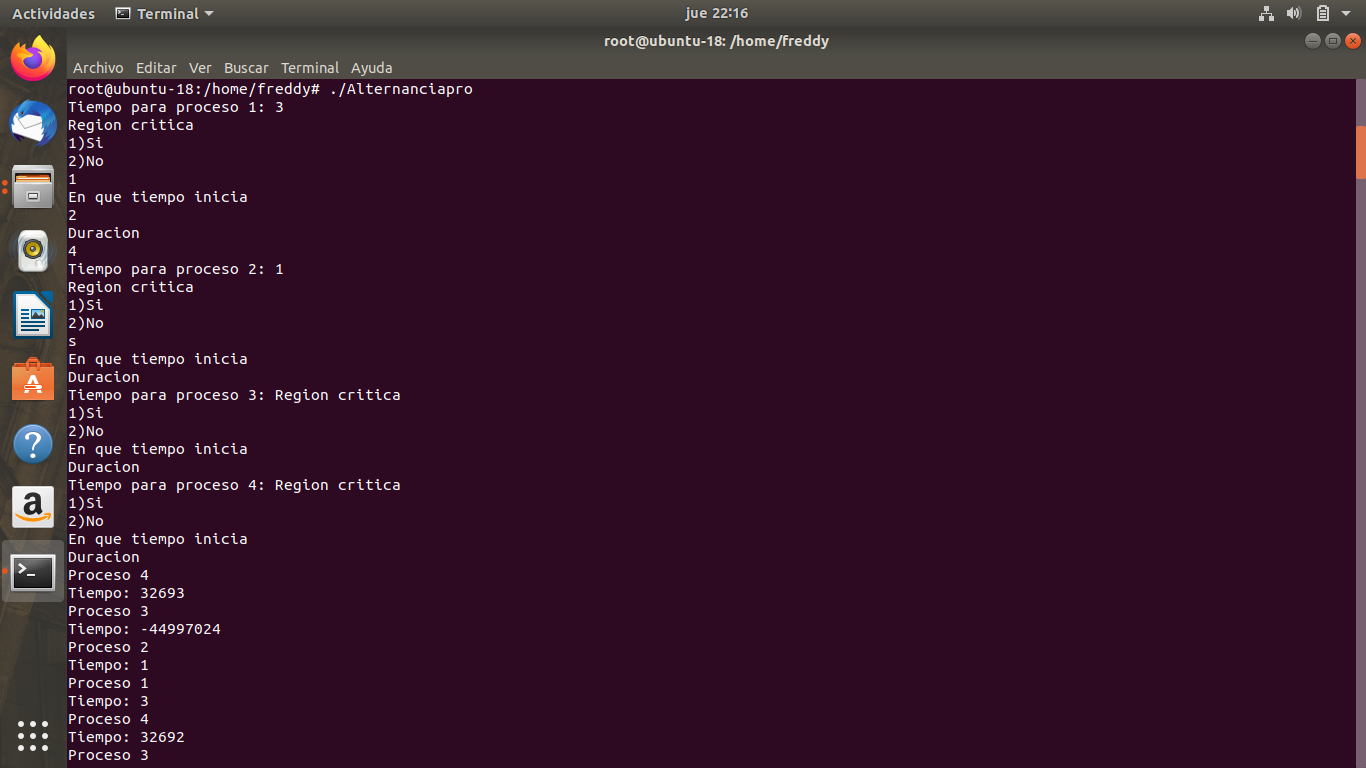
\includegraphics[scale=.35]{alternancia.png} 
\\
\\
\clearpage

\begin{lstlisting}[language=C++, caption={Comunica}]
#include <stdio.h>
#include <stdlib.h>
#include <unistd.h>
#include <sys/types.h>
#include <errno.h>
#include <signal.h>
#include <fcntl.h>
#include <sys/wait.h>
#include <ctype.h>
FILE *f;

int num_fork(int n)
{
        int i;
        for(i=1; i<n; i++)
        {
                if(fork()==0)
                {
                        return (i);
                }
        }
        return (0);
}
int main()
{
        char nombre[15];
	int cola_espera[4];
        int timpo, reg, tim_ini, tim_fin, lugar, espera;
        char r[10];
        int n, op,m,hijo;
        i=num_fork(5);
        //char *nomarchivo;
        //nomarchivo="Ids.txt";
        //remove(nomarchivo);
	printf("-----Menu-----\n");
	printf("1. Datos proceso\n");
	printf("2. Ejecuta\n");
	printf("3. Mostrar Espera");
	printf("4. Salir\n");
	scanf("%d",&op);
	switch (op)
	{
		case i:
			
	}
        switch (i)
                {
                        case 1:
					printf("Proceso uno Nombre");
                                        popen();
                                        i=getenv();
                                        fprintf(f,"Id1:%d\n",i);
                                        pclose();
                                        exit(3);

                        case 2:
                                        popen();
					i=getenv();
                                        fprintf(f,"Id2:%d\n",i);
                                        pclose();
                                        exit(3);
                        case 3:
                                        popen();
                                        i=getenv();
                                        fprintf(f,"Id3:%d\n",i);
                                        pclose();
                                        exit(3);
                        case 4:
                                        popen();
                                        i=getenv();
                                        fprintf(f,"Id4:%d\n",i);
                                        pclose();
                                        exit(3);
			default:
                                m=main(hijo);
                                m=main(hijo);
                                m=main(hijo);
                                m=main(hijo);
                                f=popen("Ids.txt","r+");
                                //printf("Valor de wwait %d",m);
                                while (fscanf(f,"%s",r) != EOF)
                                {
                                        printf("%s\n",r);

                                }
                }
}

\end{lstlisting}
\clearpage

Ejecuci\'on.\\
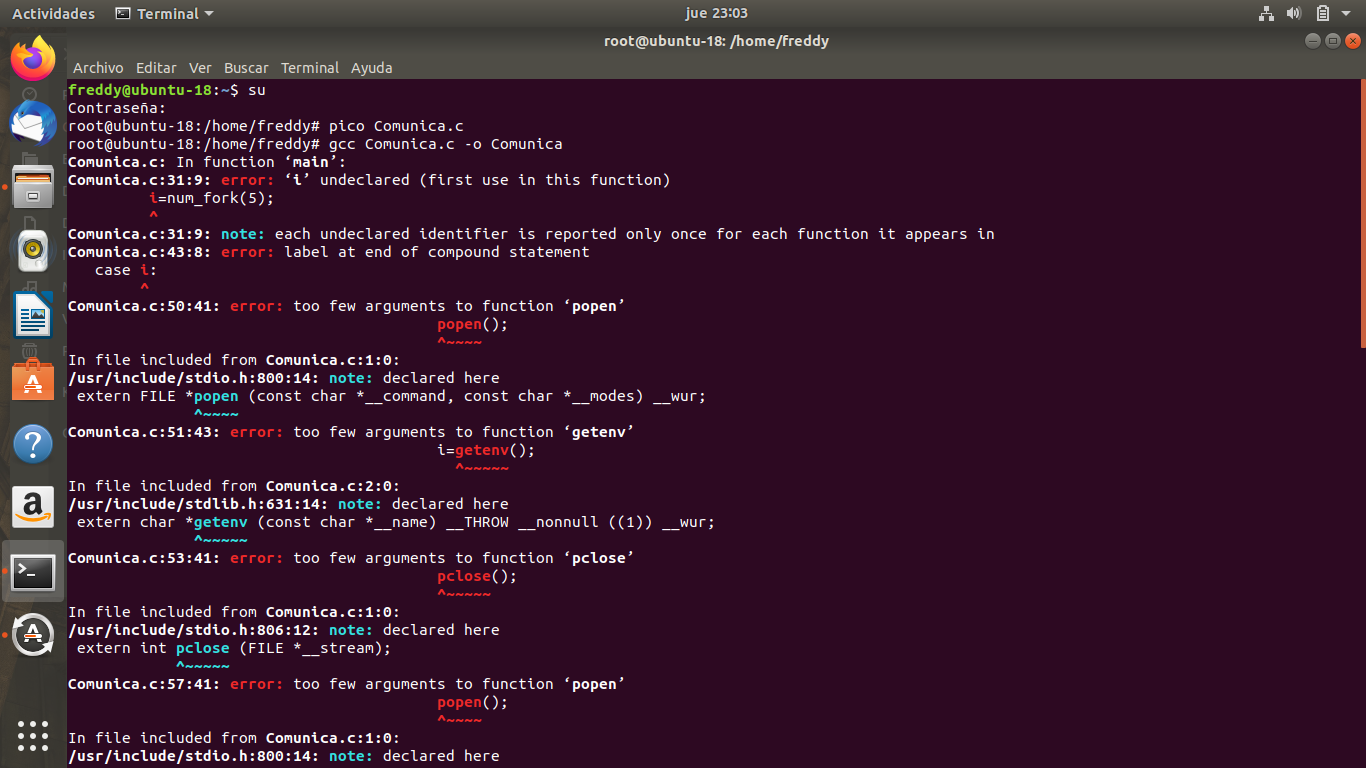
\includegraphics[scale=.35]{comunica.png} 
\\
\\
El programa de comunica no se puede ejecutar bien aunque se agregen o se cambien librerias, m\'etodos y funciones.\\

\clearpage

\begin{lstlisting}[language=C++, caption={Comunica2}]
#include <stdio.h>
#include <sys/types.h>
#include <sys/ipc.h>
#include <string.h>
#include <errno.h>
#include <unistd.h>
#include <signal.h>
#include <sys/shm.h> /* shm*  */

#define FILEKEY "/bin/cat"
#define KEY 1300
//#define NUM 10
int NUM=0;
pid_t pidL, pidM;
//int num=10;
void manejador()
{
	printf("Recibi la senal");
	kill(getpid(),SIGKILL);
	kill(pidL,SIGKILL);
	kill(pidM,SIGKILL);
}


int main ()
{
	//estructura de la senal
	struct sigaction act;
	act.sa_handler = manejador;
	sigemptyset (&act.sa_mask);
	act.sa_flags=0;
	sigaction(SIGALRM,&act,NULL);
	alarm(3);
	//Declaracion de variables
	int fd[2];
	int key, i;
        int id_zone;
        int *buffer;
        char c;
	char a;
        pipe(fd);//Creacion de tuberia
	/*El proceso padre crea la memoria compartida para la sincronizacion 
	de los procesos*/
        //LLava e para la memoria compartida
        key = ftok(FILEKEY, KEY);//crea la llave
        if (key == -1)//Si no s epude crear la llave
        {
                //Despliega letrero
                fprintf (stderr, "Error al crear la llave \n");
                return -1;
        }
        //Crea la memoria compartida
        id_zone = shmget (key, sizeof(int)*NUM, 0777 | IPC_CREAT);
        if (id_zone == -1)//Si no se pudo crear la memoria
        {
                //Despliega letrero
                fprintf (stderr, "Error al crear memoria compartida\n");
                return -1;
        }
        //printf ("ID zone shared memory: %i\n", id_zone);
        //Imprime el ID de la zona
        //Ata memoria compartida
        buffer = shmat (id_zone, (char *)0, 0);
        if (buffer == NULL)//Si no se puede atar la memoria
        {
             //Imprime error
             fprintf (stderr, "Error al reservar memoria compartida \n");
              return -1;
        }
       //printf ("Puntero al buffer de la memoria compartida %p\n", buffer);
       //Imprim el puntero
	//printf("Soy el prceso R \t Mi ID es: %d\n",getpid());
	pipe(fd);//Creacion de tuberia
	pidL = fork();//Cracion de proceso L
	if (pidL == 0)//Si se creo el proceso L
	{
	/*Crea memoria compartida para modificar variable compartida, incrementa
     variable*/
		//printf("Proceso hijo %d intentando entrar a memoria",getpid());
                int key, i, id_zone, *buffer;
                /*LLave para memoria compartida */
                key = ftok(FILEKEY, KEY);
                if (key == -1)
                {
                        fprintf (stderr, "Error al crear llave \n");
                	return -1;
                }
                /* Se crea la memoria comartida*/
                id_zone = shmget (key, sizeof(int)*NUM, 0777 | IPC_CREAT);
                if (id_zone == -1)
                {
                     fprintf (stderr, "Error al crear memoria compartida\n");
                     return -1;
                }
                //printf ("ID de la zona de memoria compartida: %i\n", id_zone);
                /* Declaracion de la memoria compartida */
                buffer = shmat (id_zone, (char *)0, 0);
                if (buffer == NULL)
                {
                     fprintf (stderr, "Error al reservar memoria compartida \n");
                     return -1;
                }

        //printf ("Puntero del buffer de la memoria compartida: %p\n", buffer);
		while(1)
		{
			//printf(" %d\t",getpid());
			NUM++;
			write(fd[1],&NUM,sizeof(int));
		}
	}
	pidM = fork();//Proceso de proceso M
	if (pidM == 0)
	{
/*Crea memoria compartida para modificar variable compartida,decrementa variable*/
            //printf("Proceso hijo %d intentando entrar a memoria",getpid());
                int key, i, id_zone, *buffer;
                /*LLave para memoria compartida */
                key = ftok(FILEKEY, KEY);
                if (key == -1)
                {
                        fprintf (stderr, "Error al crear llave \n");
                        return -1;
                }
                /* Se crea la memoria comartida*/
                id_zone = shmget (key, sizeof(int)*NUM, 0777 | IPC_CREAT);
                if (id_zone == -1)
                {
                        fprintf (stderr, "Error al crear memoria compartida\n");
                        return -1;
                }
                //printf ("ID de la zona de memoria compartida: %i\n", id_zone);
                /* Declaracion de la memoria compartida */
                buffer = shmat (id_zone, (char *)0, 0);
                if (buffer == NULL)
                {
                      fprintf (stderr, "Error al reservar memoria compartida \n");
                      return -1;
                }
             //printf ("Puntero del buffer de la memoria compartida:
              %p\n", buffer);
		while(1)
		{
			//printf(" %d\t",getpid());
			NUM--;
			write(fd[1],&NUM,sizeof(int));
		}
	}
	while (1)//Imprime los datos a pantalla 
	{
		//printf("Soy el prceso padre \t Mi ID es: %d\n",getpid());
		read(fd[0],&NUM,sizeof(int));
		printf("%d\n",NUM);
		read(fd[0],&NUM,sizeof(int));
		printf("%d\n",NUM);
	}
	c = getchar();
        //libera la memoria compartida
        shmdt ((char *)buffer);
        shmctl (id_zone, IPC_RMID, (struct shmid_ds *)NULL);
        return 0;

}

\end{lstlisting}
Ejecuci\'on.\\
\includegraphics[scale=.35]{Comunica2.png} 
\\
\\
En el programa comunica2 se ejecuta y nos da como salida un error para crear memoria compartida.
\clearpage

\begin{lstlisting}[language=C++, caption={Ejem}]
#include <stdio.h>
#include <sys/types.h>
#include <sys/ipc.h>
#include <string.h>
#include <errno.h>
#include <sys/shm.h> /* shm*  */
#include<unistd.h>


#define FILEKEY "/bin/cat"
#define KEY 1300
#define MAXBUF 10



int main ()
{
        int key, i;
        int id_zone;
        int *buffer;
        char c;
	pid_t pid1;
        //LLava e para la memoria compartida
        key = ftok(FILEKEY, KEY);
        if (key == -1)
        {
                fprintf (stderr, "Error al crear la llave \n");
                return -1;
        }
	//Crea la memoria compartida
        id_zone = shmget (key, sizeof(int)*MAXBUF, 0777 | IPC_CREAT);
        if (id_zone == -1)
        {
                fprintf (stderr, "Error al crear memoria compartida\n");
                return -1;
                return -1;
        }
        printf ("ID zone shared memory: %i\n", id_zone);
        //Declarar memoria compartida
        buffer = shmat (id_zone, (char *)0, 0);
        if (buffer == NULL)
        {
                fprintf (stderr, "Error al reservar memoria compartida \n");
                return -1;
        }
        printf ("Puntero al buffer de la memoria compartida %p\n", buffer);
        for (i = 0; i < MAXBUF; i++)
        {
                buffer[i] = i;
        }
	pid1=fork();
	//Crea un hijo para entrar en memria compartida.
	if (pid1 == 0)
	{
		printf("Proceso hijo %d intentando entrar a memoria",getpid());
		int key, i, id_zone, *buffer;
        	/*LLave para memoria compartida */
	        key = ftok(FILEKEY, KEY);
	        if (key == -1)
	        {
	                fprintf (stderr, "Error al crear llave \n");
	        return -1;
        	}
		        /* Se crea la memoria comartida*/
	        id_zone = shmget (key, sizeof(int)*MAXBUF, 0777 | IPC_CREAT);
	        if (id_zone == -1)
	        {
	                fprintf (stderr, "Error al crear memoria compartida\n");
	                return -1;
        	}

	        printf ("ID de la zona de memoria compartida: %i\n", id_zone);
        	/* Declaracion de la memoria compartida */
		buffer = shmat (id_zone, (char *)0, 0);
	        if (buffer == NULL)
	        {
	                fprintf (stderr, "Error al reservar memoria compartida \n");
	                return -1;
	        }

	        printf ("Puntero del buffer de la memoria compartida: %p\n", buffer);
	        /* Escribe los valores a la memoria */
	        for (i = 0; i < MAXBUF; i++)
	        {
	                printf ("%i\n", buffer[i]);
	        }
		//printf("Proceso hijo %d intentando entrar a memoria",getpid());
	}
        c = getchar();
        //libera la memoria compartida
        shmdt ((char *)buffer);
	shmctl (id_zone, IPC_RMID, (struct shmid_ds *)NULL);
        return 0;
}

\end{lstlisting}
\clearpage
Ejecuci\'on\\
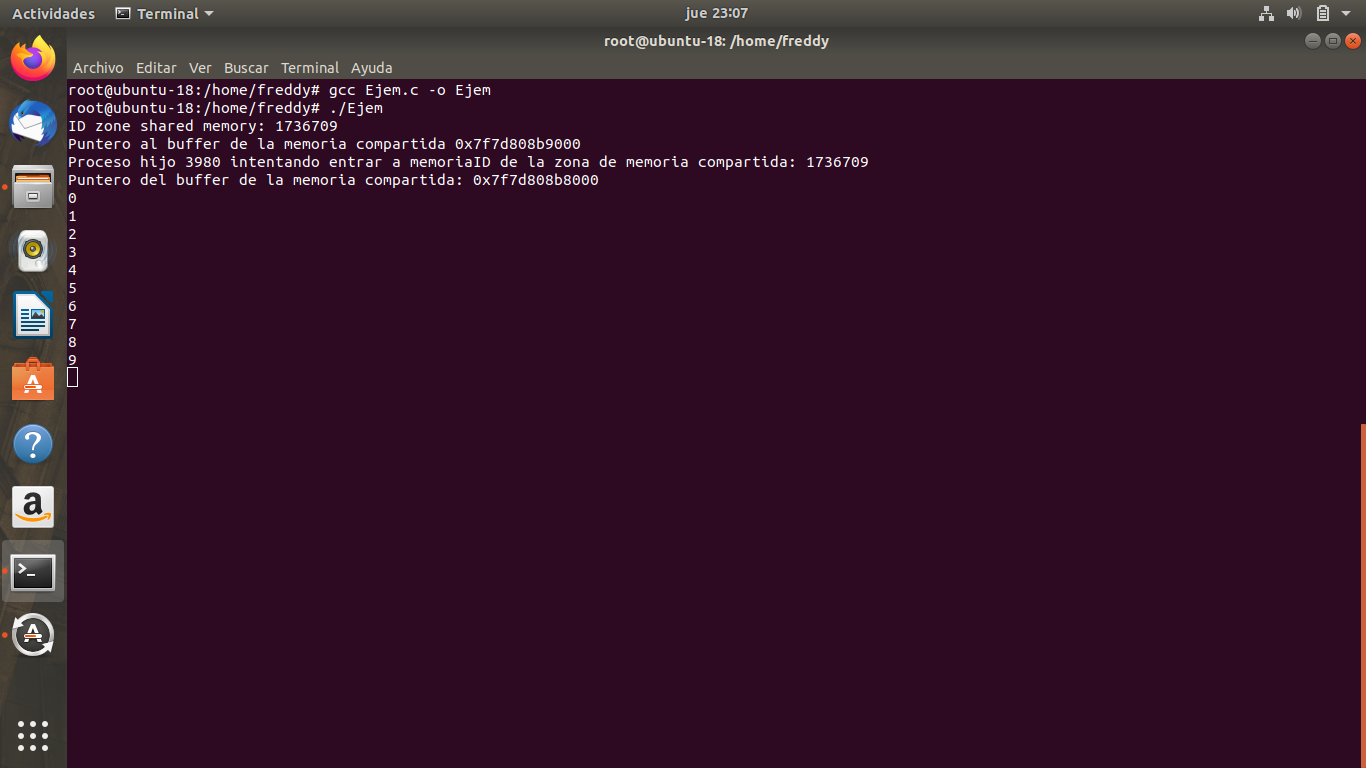
\includegraphics[scale=.35]{Ejem.png}
\\
\\
Nuestro programa ejecuta la funcion de crear un puntero en el buffer para la memoria compartida
\clearpage

\begin{lstlisting}[language=C++, caption={Ejem.men}]
#include <stdio.h>
#include <sys/types.h>
#include <sys/ipc.h>
#include <string.h>
#include <errno.h>
#include <sys/shm.h> /* shm*  */

#define FILEKEY "/bin/cat"
#define KEY 1300
#define MAXBUF 10



int main ()
{
        int key, i;
        int id_zone;
        int *buffer;
        char c;
	pid_t pid1;
        //LLava e para la memoria compartida
        key = ftok(FILEKEY, KEY);
        if (key == -1)
        {
                fprintf (stderr, "Error al crear la llave \n");
                return -1;
        }
	//Crea la memoria compartida
        id_zone = shmget (key, sizeof(int)*MAXBUF, 0777 | IPC_CREAT);
        if (id_zone == -1)
        {
                fprintf (stderr, "Error al crear memoria compartida\n");
                return -1;
                return -1;
        }
        printf ("ID zone shared memory: %i\n", id_zone);
        //Declarar memoria compartida
        buffer = shmat (id_zone, (char *)0, 0);
        if (buffer == NULL)
        {
                fprintf (stderr, "Error al reservar memoria compartida \n");
                return -1;
        }
        printf ("Puntero al buffer de la memoria compartida %p\n", buffer);
        for (i = 0; i < MAXBUF; i++)
        {
                buffer[i] = i;
        }
	pid1=fork();
	//Crea un hijo para entrar en memria compartida.
	if (pid1 == 0)
	{
		printf("Proceso hijo %d intentando entrar a memoria",getpid());
		int key, i, id_zone, *buffer;
        	/*LLave para memoria compartida */
	        key = ftok(FILEKEY, KEY);
	        if (key == -1)
	        {
	                fprintf (stderr, "Error al crear llave \n");
	        return -1;
        	}
		        /* Se crea la memoria comartida*/
	        id_zone = shmget (key, sizeof(int)*MAXBUF, 0777 | IPC_CREAT);
	        if (id_zone == -1)
	        {
	                fprintf (stderr, "Error al crear memoria compartida\n");
	                return -1;
        	}

	        printf ("ID de la zona de memoria compartida: %i\n", id_zone);
        	/* Declaracion de la memoria compartida */
		buffer = shmat (id_zone, (char *)0, 0);
	        if (buffer == NULL)
	        {
	                fprintf (stderr, "Error al reservar memoria compartida \n");
	                return -1;
	        }

	        printf ("Puntero del buffer de la memoria compartida: %p\n", buffer);
	        /* Escribe los valores a la memoria */
	        for (i = 0; i < MAXBUF; i++)
	        {
	                printf ("%i\n", buffer[i]);
	        }
		//printf("Proceso hijo %d intentando entrar a memoria",getpid());
	}
        c = getchar();
        //libera la memoria compartida
        shmdt ((char *)buffer);
	shmctl (id_zone, IPC_RMID, (struct shmid_ds *)NULL);
        return 0;
}

\end{lstlisting}
Ejecuci\'on\\
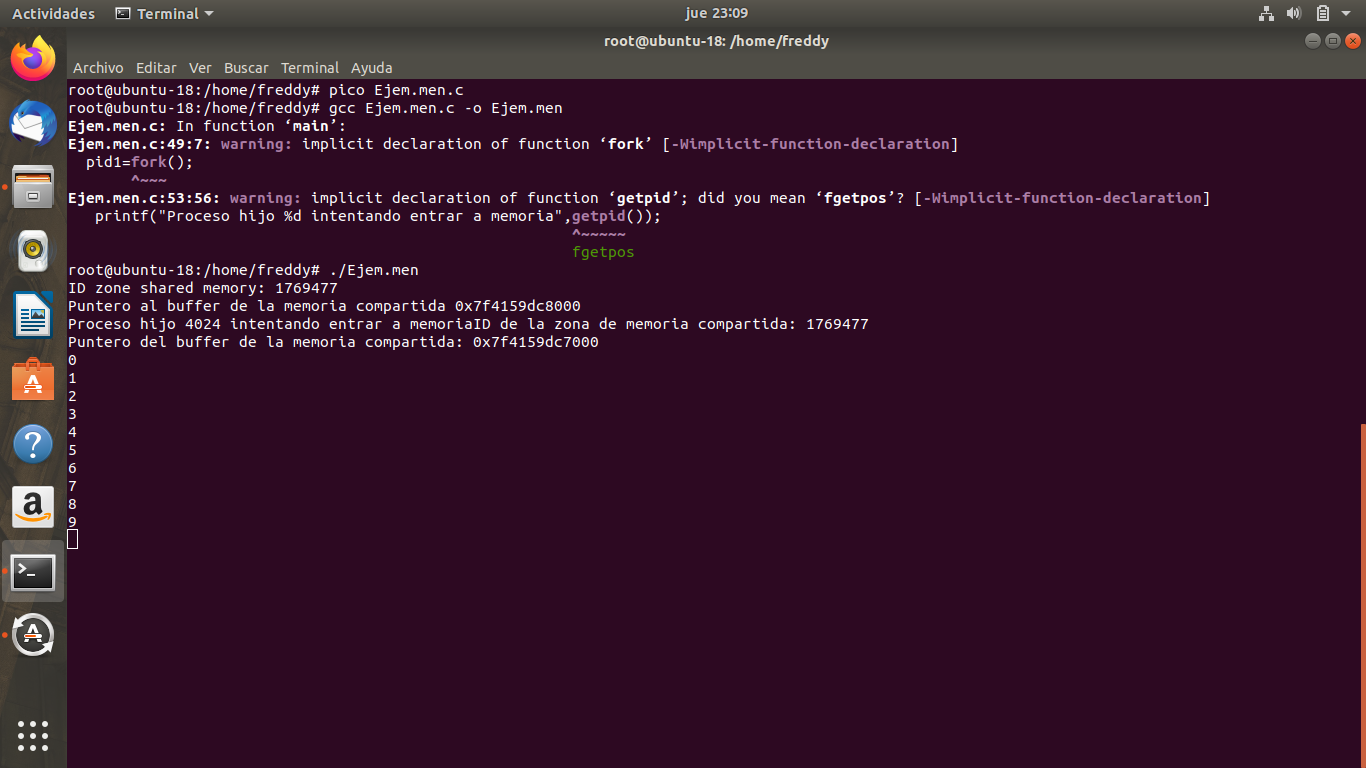
\includegraphics[scale=0.3]{ejem0.png}  
\\
Puntero de memoria compartida, en la cual el proceso hijo intenta entar a la memoria compartida
\clearpage
\begin{lstlisting}[language=C++, caption={Ejem.tub1}]
#include <stdio.h>
#include <sys/types.h>
#include <sys/ipc.h>
#include <string.h>
#include <errno.h>
#include <unistd.h>
#include <signal.h>
#include <sys/shm.h> /* shm*  */

#define FILEKEY "/bin/cat"
#define KEY 1300
//#define NUM 10
int NUM=0;
pid_t pidL, pidM;
//int num=10;
void manejador()
{
	printf("Recibi la senal");
	kill(getpid(),SIGKILL);
	kill(pidL,SIGKILL);
	kill(pidM,SIGKILL);
}


int main ()
{
	//estructura de la senal
	struct sigaction act;
	act.sa_handler = manejador;
	sigemptyset (&act.sa_mask);
	act.sa_flags=0;
	sigaction(SIGALRM,&act,NULL);
	alarm(3);
	//Declaracion de variables
	int fd[2];
	int key, i;
        int id_zone;
        int *buffer;
        char c;
	char a;
        pipe(fd);//Creacion de tuberia
	/*El proceso padre crea la memoria compartida para la sincronizacion
	 de los procesos*/
        //LLava e para la memoria compartida
        key = ftok(FILEKEY, KEY);//crea la llave
        if (key == -1)//Si no s epude crear la llave
        {
            //Despliega letrero
            fprintf (stderr, "Error al crear la llave \n");
                return -1;
        }
        //Crea la memoria compartida
        id_zone = shmget (key, sizeof(int)*NUM, 0777 | IPC_CREAT);
        if (id_zone == -1)//Si no se pudo crear la memoria
        {
                //Despliega letrero
                fprintf (stderr, "Error al crear memoria compartida\n");
                return -1;
        }
        //printf ("ID zone shared memory: %i\n", id_zone);
        //Imprime el ID de la zona
        //Ata memoria compartida
        buffer = shmat (id_zone, (char *)0, 0);
        if (buffer == NULL)//Si no se puede atar la memoria
        {
              //Imprime error
              fprintf (stderr, "Error al reservar memoria compartida \n");
                return -1;
        }
    //printf ("Puntero al buffer de la memoria compartida %p\n", buffer);
    //Imprim el puntero
	//printf("Soy el prceso R \t Mi ID es: %d\n",getpid());
	pipe(fd);//Creacion de tuberia
	pidL = fork();//Cracion de proceso L
	if (pidL == 0)//Si se creo el proceso L
	{
		/*Crea memoria compartida para modificar variable compartida,
		 incrementa variable*/
		//printf("Proceso hijo %d intentando entrar a memoria",getpid());
                int key, i, id_zone, *buffer;
                /*LLave para memoria compartida */
                key = ftok(FILEKEY, KEY);
                if (key == -1)
                {
                        fprintf (stderr, "Error al crear llave \n");
                	return -1;
                }
                /* Se crea la memoria comartida*/
                id_zone = shmget (key, sizeof(int)*NUM, 0777 | IPC_CREAT);
                if (id_zone == -1)
                {
                     fprintf (stderr, "Error al crear memoria compartida\n");
                     return -1;
                }
              //printf ("ID de la zona de memoria compartida: %i\n", id_zone);
              /* Declaracion de la memoria compartida */
                buffer = shmat (id_zone, (char *)0, 0);
                if (buffer == NULL)
                {
                     fprintf (stderr, "Error al reservar memoria compartida \n");
                    return -1;
                }

        //printf ("Puntero del buffer de la memoria compartida: %p\n", buffer);
		while(1)
		{
			//printf(" %d\t",getpid());
			NUM++;
			write(fd[1],&NUM,sizeof(int));
		}
	}
	pidM = fork();//Proceso de proceso M
	if (pidM == 0)
	{
		/*Crea memoria compartida para modificar variable compartida, 
		decrementa variable*/
        //printf("Proceso hijo %d intentando entrar a memoria",getpid());
                int key, i, id_zone, *buffer;
                /*LLave para memoria compartida */
                key = ftok(FILEKEY, KEY);
                if (key == -1)
                {
                        fprintf (stderr, "Error al crear llave \n");
                        return -1;
                }
                /* Se crea la memoria comartida*/
                id_zone = shmget (key, sizeof(int)*NUM, 0777 | IPC_CREAT);
                if (id_zone == -1)
                {
                    fprintf (stderr, "Error al crear memoria compartida\n");
                    return -1;
                }
              //printf ("ID de la zona de memoria compartida: %i\n", id_zone);
              /* Declaracion de la memoria compartida */
                buffer = shmat (id_zone, (char *)0, 0);
                if (buffer == NULL)
                {
                    fprintf (stderr, "Error al reservar memoria compartida \n");
                    return -1;
                }
         //printf ("Puntero del buffer de la memoria compartida: %p\n", buffer);
		while(1)
		{
			//printf(" %d\t",getpid());
			NUM--;
			write(fd[1],&NUM,sizeof(int));
		}
	}
	while (1)//Imprime los datos a pantalla 
	{
		//printf("Soy el prceso padre \t Mi ID es: %d\n",getpid());
		read(fd[0],&NUM,sizeof(int));
		printf("%d\n",NUM);
		read(fd[0],&NUM,sizeof(int));
		printf("%d\n",NUM);
	}
	c = getchar();
        //libera la memoria compartida
        shmdt ((char *)buffer);
        shmctl (id_zone, IPC_RMID, (struct shmid_ds *)NULL);
        return 0;

}

\end{lstlisting}
Ejecuci\'on\\
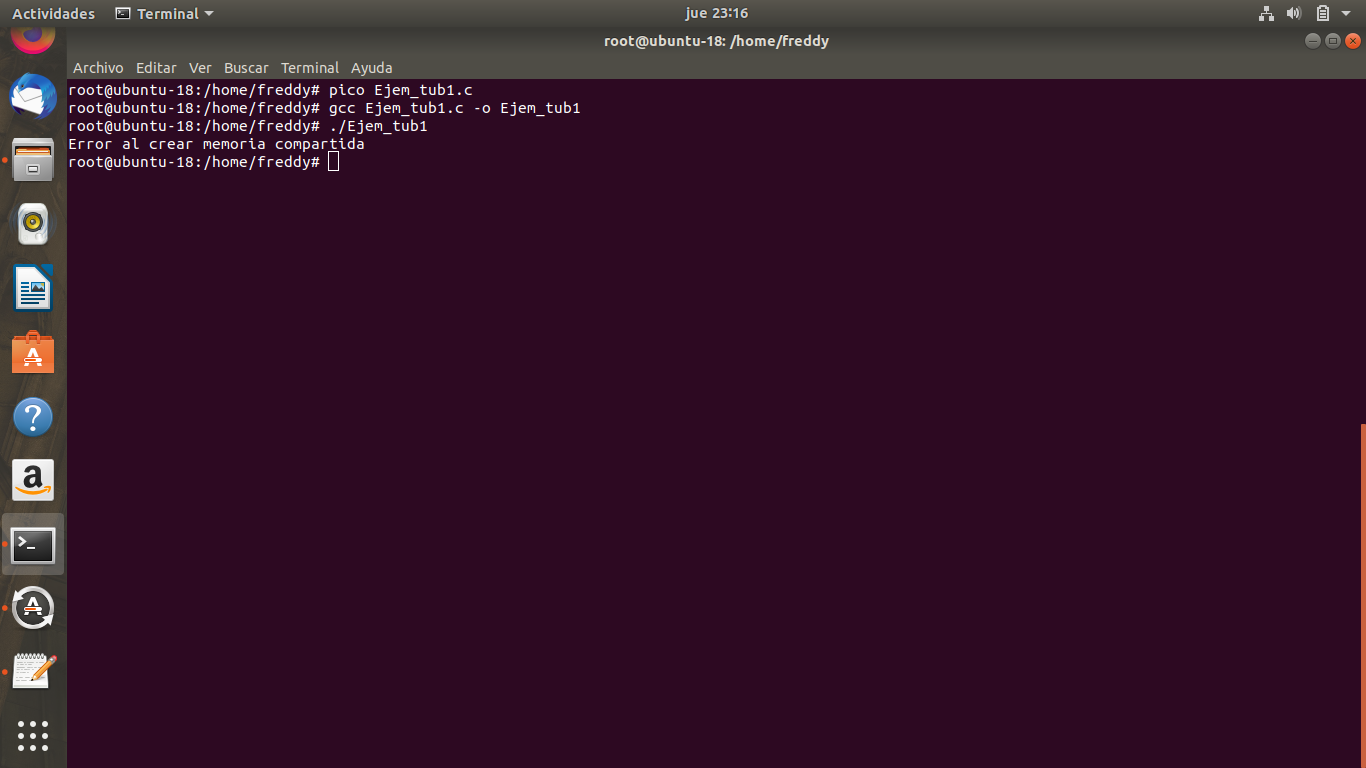
\includegraphics[scale=.35]{ejem_tub1.png}
\\
\\
Error al crear la memoria compartida mediante un programa tipo tuberia
\clearpage
\begin{lstlisting}[language=C++, caption={Ejem1}]
#include <stdio.h>
#include <sys/types.h>
#include <sys/ipc.h>
#include <sys/shm.h>
#include <sys/wait.h>
#include<unistd.h>

int main()
{
	pid_t pid1,pid2;
	pid1=fork();
	if(pid1>0){
		pid2=fork();
		if(pid2>0){//Padre C
			int id,*ap,status,c[15],suma,i;
			suma=0;
			wait(&status);
			wait(&status);
			id=shmget(ftok(".",'&'),sizeof(c),IPC_CREAT);
			ap=shmat(id,0,0);
			for(i=0;i<15;i++){
				printf("ap %d: %d\n",i,*ap+i);
				suma+=*(ap+i);
			}
			shmdt(ap);
			shmctl(id,IPC_RMID,NULL);
			id=shmget(ftok(".",'%'),sizeof(int),IPC_CREAT);
			ap=shmat(id,0,0);
			*ap=suma;
		}
		if(pid2==0){//Hijo B
			int id,*ap,B[15],i;
			id=shmget(ftok(".",'&'),sizeof(B),IPC_CREAT);
			ap=shmat(id,0,0);
			for(i=1;i<=15;i+=2){
				//*(ap+i)=i;
				*(ap+i)=(100);
			}
		}
	}
	if(pid1==0){//Hijo A
		int id,*ap,B[15],i;
		id=shmget(ftok(".",'&'),sizeof(B),IPC_CREAT);
		ap=shmat(id,0,0);
		for(i=0;i<15;i+=2){
			//*(ap+i)=i;
			*(ap+i)=(100);
		}
	}
}
\end{lstlisting}
\clearpage
Ejecuci\'on\\
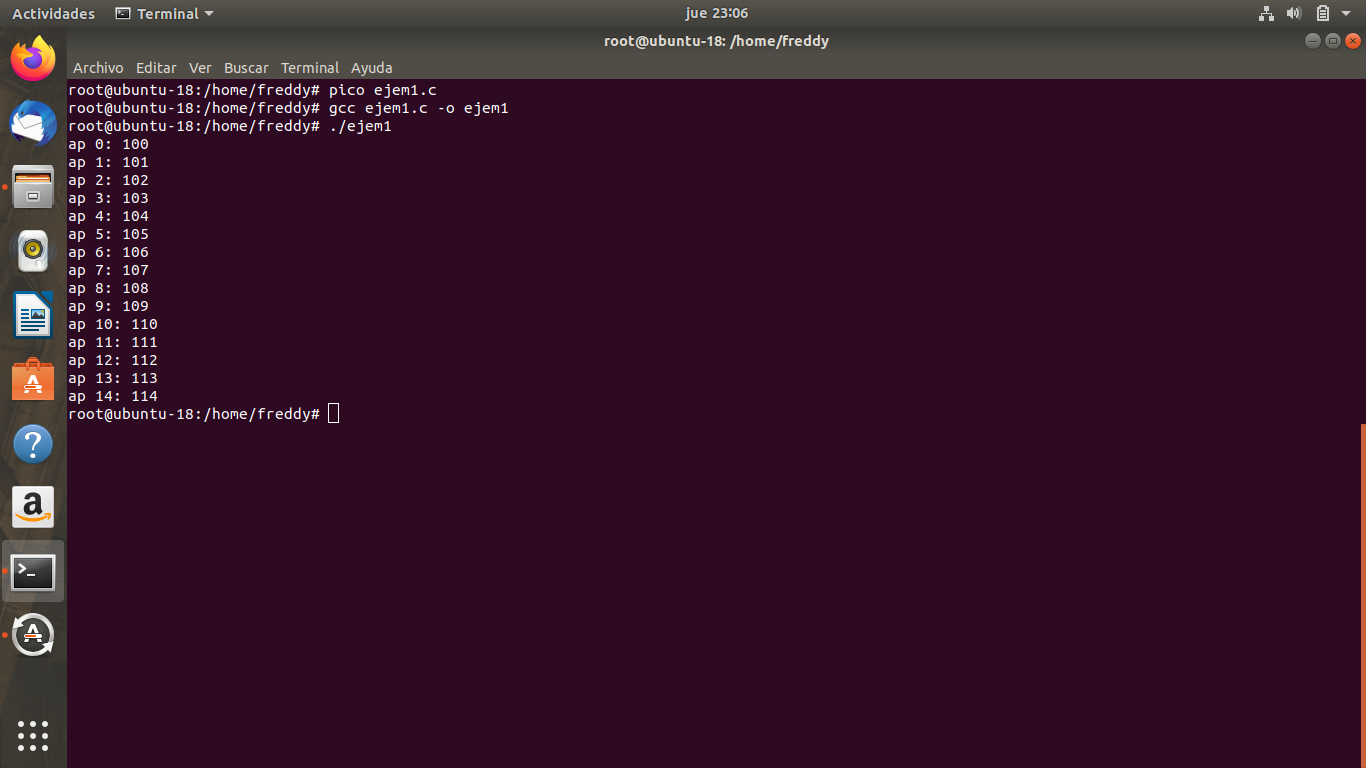
\includegraphics[scale=.35]{ejem1.png}
\\
\\
Creando padre e hijos mediante tuberias
\clearpage
\begin{lstlisting}[language=C++, caption={Ejemplo2}]
#include <stdio.h>
#include <sys/types.h>
#include <sys/ipc.h>
#include <sys/shm.h>

int main(){
	int id, *ap;
	id=shmget(ftok(".",'%'),sizeof(int),IPC_CREAT);
	ap=shmat(id,0,0);
	printf("Suma: %d\n",*ap);
}
\end{lstlisting}
Ejecuci\'on\\
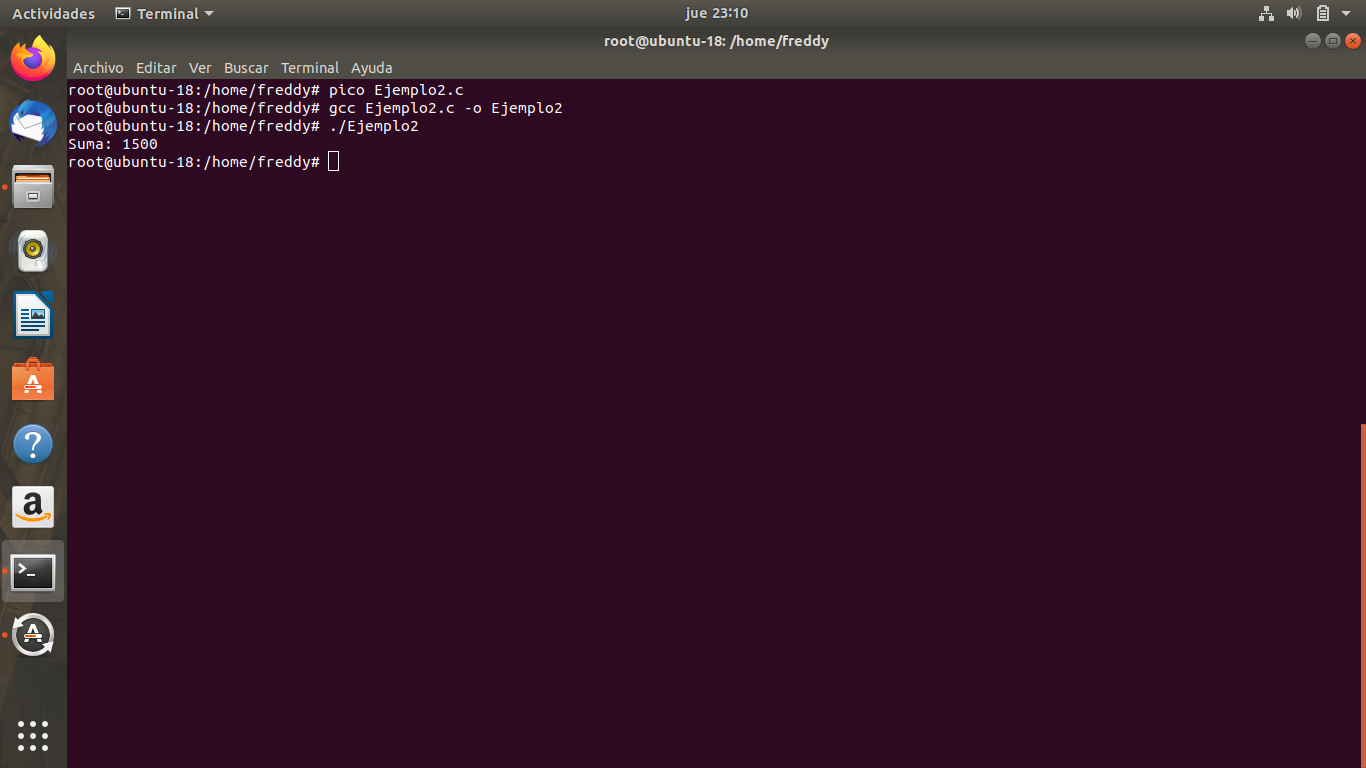
\includegraphics[scale=.35]{ejemplo2.png}
\\
\\
Este programa calcula la suma mediante funcion shmget
\clearpage
\begin{lstlisting}[language=C++, caption={Ejemtub1}]
#include <stdio.h>
#include <stdlib.h>
#include <sys/types.h>
#include <signal.h>
#include<unistd.h>

void GeneraPares(int tuberia, int t1, int t2)
{
	int i=0;
	char testigo;
	/*i es el numero par que se genera*/
	/*Se geenera el primer lugar el 0*/
	write(tuberia, &i, sizeof(const void));
	/*Sede el turno a p2*/
	write(t1, testigo, sizeof(const void));
	for(i=0; i < 2000; i=i+2)
	{
		/*Espera el turno*/
		read(t2, testigo, sizeof(void));
		/*Inserta el siguiente numero par*/
		write(tuberia, &i, sizeof(const void));
		/*Cede el turnoa p2*/
		write(t1, &testigo, sizeof(const void));

	}
	return;
}

void GeneraImpares(int tuberia, int t1, int t2)
{
	int i=0;
	char testigo;
	/*i es el numero impar que se ogenera*/
	for(i=1; i<2000; i=i+2)
	{
		/*Espera el turno */
		read(t1, &testigo, sizeof(void));
		/*Inserta el ssiguieente numero par*/
		write(tuberia, &i, sizeof(const void));
		/*Cede el turno al p1*/
		write(t2, &testigo, sizeof(const void));
	}
	return;
}

void ConsumeNumeros(int tuberia)
{
	int i;
	while(read(tuberia, &i, sizeof(int)) > 0)
	{
		/*Escribe el caracter*/
		printf("%d\n",i);
	}
	return;
}

int main ()
{
	pid_t pid1, pid2;
	/*Tuberia ocupada como sisstema dde comunicacion*/
	/*Entre los tres procesos*/
	int tuberia[2];

	/*Tuberias utilizadas para sincronizar a los procesos p1 y p2*/
	int t1[2], t2[2];
	/*El proceso padre sera el que cree la tuberia*/
	if (pipe(tuberia) < 0)
	{
		perror("No se puede crear la tuberia");
		exit(0);
	}
	if (pipe(t1) < 0)
	{
		perror("No se puede crear la tuberia");

		exit(0);
	}
	if(pipe(t2) < 0)
	{
		perror("No se puede crear la tuberia");
	}
	/*Se crea elproceso p1*/
	switch(pid1=fork())
	{
		case -1:
			perror("No se pued crear el proceso");
			/*Se ciierra la pipe*/
			close(tuberia[0]);
			close(tuberia[1]);
			close(t1[0]);
			close(t1[1]);
			close(t2[0]);
			close(t2[1]);
			exit(0);
		case 0: /*Proceso hijo proceso p1*/
			/*Cierra el descriptor de lecura de la pipe*/
			close(tuberia[0]);
			/*Este proceso lee de t1 y escribe en t2*/
			close(t1[1]);
			close(t2[0]);
			GeneraImpares(tuberia[1], t1[0], t2[1]);
			/*El  proceso acaba los descriptores*/
			close(tuberia[1]);
			close(t1[0]);
			close(t2[1]);
			break;
		default:
			/*El proceso padre crea ahora el proceso p2*/
			switch(pid2 = fork())
			{
				case -1:
					perror("Error al crear el proceso p2");
					/*Se ciierra la pipe*/
                        		close(tuberia[0]);
		                        close(tuberia[1]);
                		        close(t1[0]);
		                        close(t1[1]);
		                        close(t2[0]);
		                        close(t2[1]);
					/*Se mata el proceso anterior*/
					kill(pid1, SIGKILL);
					exit(0);
				case 0:/*Proceso hijo p2*/
					/*lee de la tuberia*/
					/*Cierra el descriptor de escritura*/
					close(tuberia[1]);
					/*no necesita t1 ni t2*/
					close(t1[0]);
                                        close(t1[1]);
                                        close(t2[0]);
                                        close(t2[1]);
					ConsumeNumeros(tuberia[0]);
					close(tuberia[0]);
					exit(0);
					break;
				default:/*Procesoo padre*/
					/*Escribe en la tuberia*/
					/*Cierra el descriptor de lectura*/
					close(tuberia[0]);
					/*Este proceso lee de t2*/
					/*y escribe en t1.Cierra lo que no necesita*/
					close(t1[0]);
					close(t2[1]);
					GeneraImpares(tuberia[1], t1[1], t2[0]);
					/*El proceso cierra los descriptores*/
					close(tuberia[1]);
					close(t1[1]);
					close(t2[0]);
			}
	}
}
\end{lstlisting}
\clearpage
Ejecuci\'on\\
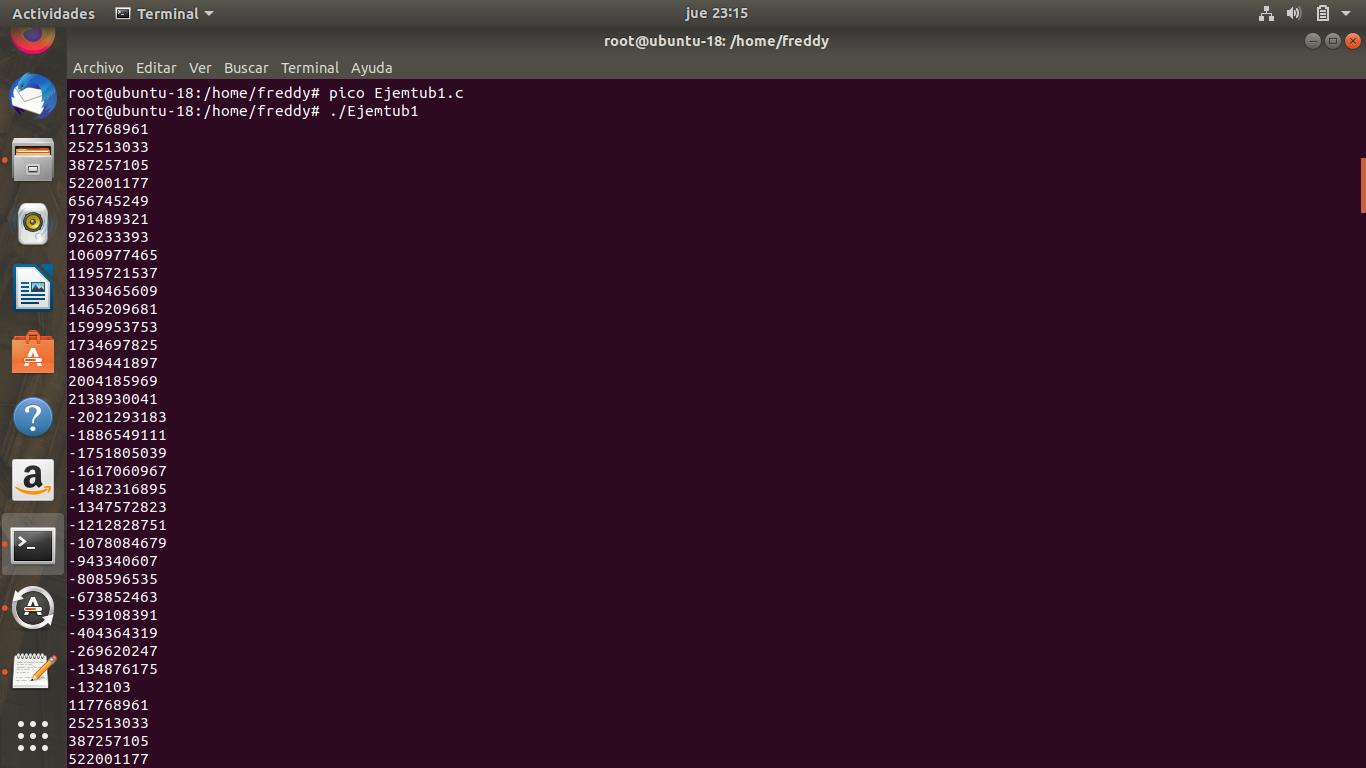
\includegraphics[scale=.35]{ejemtub1.png}
\\
\\
Este programa crea tuberias, los manda a llamar, pero si esta ocupada la tuberia llama a otra, se utiliza para sincronizar procesos entre tuberias, al igual crea procesos padre e hijos y puede matar los procesos creados.
\clearpage
\begin{lstlisting}[language=C++, caption={pro2}]
#include <stdio.h>
#include <sys/types.h>
#include <sys/ipc.h>
#include <string.h>
#include <errno.h>
#include <sys/shm.h> /* shm*  */

#define FILEKEY "/bin/cat"
#define KEY 1300
#define MAXBUF 10

int main ()
{
	int key, i, id_zone, *buffer;
   	/*LLave para memoria compartida */
	key = ftok(FILEKEY, KEY);
   	if (key == -1)
	{
		fprintf (stderr, "Error al crear llave \n");
      	return -1;
   	}

   	/* Se crea la memoria comartida*/
   	id_zone = shmget (key, sizeof(int)*MAXBUF, 0777 | IPC_CREAT);
   	if (id_zone == -1)
	{
      		fprintf (stderr, "Error al crear memoria compartida\n");
      		return -1;
   	}

   	printf ("ID de la zona de memoria compartida: %i\n", id_zone);
   	/* Declaracion de la memoria compartida */
   	buffer = shmat (id_zone, (char *)0, 0);
   	if (buffer == NULL)
	{
      		fprintf (stderr, "Error al reservar memoria compartida \n");
      		return -1;
   	}


	printf ("Puntero del buffer de la memoria compartida: %p\n", buffer);
   	/* Escribe los valores a la memoria */
   	for (i = 0; i < MAXBUF; i++)
	{
      		printf ("%i\n", buffer[i]);
	}
   	return 0;
}
\end{lstlisting}
\clearpage
Ejecuci\'on\\
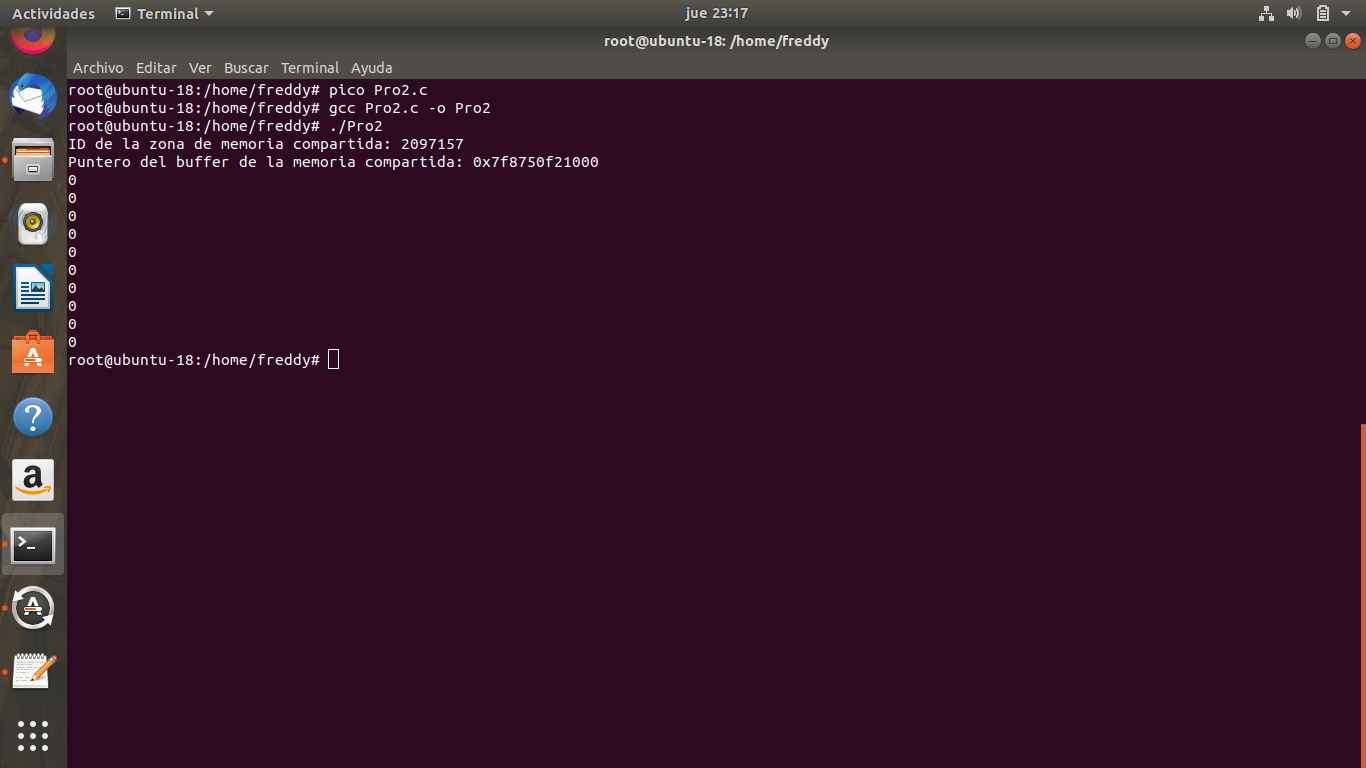
\includegraphics[scale=.35]{pro2.png}
\\
\\
Creando llave para memoria compartida entrando a la zona de memoria
\clearpage
\begin{lstlisting}[language=C++, caption={Proc1}]
#include <stdio.h>
#include <sys/types.h>
#include <sys/ipc.h>
#include <string.h>
#include <errno.h>
#include <sys/shm.h> /* shm*  */

#define FILEKEY "/bin/cat"
#define KEY 1300
#define MAXBUF 10



int main ()
{
	int key, i;
	int id_zone;
	int *buffer;
	char c;
	//LLava e para la memoria compartida
	key = ftok(FILEKEY, KEY);
	if (key == -1)
	{
		fprintf (stderr, "Error al crear la llave \n");
		return -1;
	}
	//Crea la memoria compartida
	id_zone = shmget (key, sizeof(int)*MAXBUF, 0777 | IPC_CREAT);
	if (id_zone == -1)
	{
		fprintf (stderr, "Error al crear memoria compartida\n");
	      	return -1;
   	}
	printf ("ID zone shared memory: %i\n", id_zone);
   	//Declarar memoria compartida
   	buffer = shmat (id_zone, (char *)0, 0);
   	if (buffer == NULL)
	{
	      	fprintf (stderr, "Error al reservar memoria compartida \n");
      		return -1;
	}
   	printf ("Puntero al buffer de la memoria compartida %p\n", buffer);
	for (i = 0; i < MAXBUF; i++)
	{
		buffer[i] = i;
	}
	c = getchar();
   	//libera la memoria compartida
	shmdt ((char *)buffer);
	shmctl (id_zone, IPC_RMID, (struct shmid_ds *)NULL);
   	return 0;
}
\end{lstlisting}
\clearpage
Ejecuci\'on\\
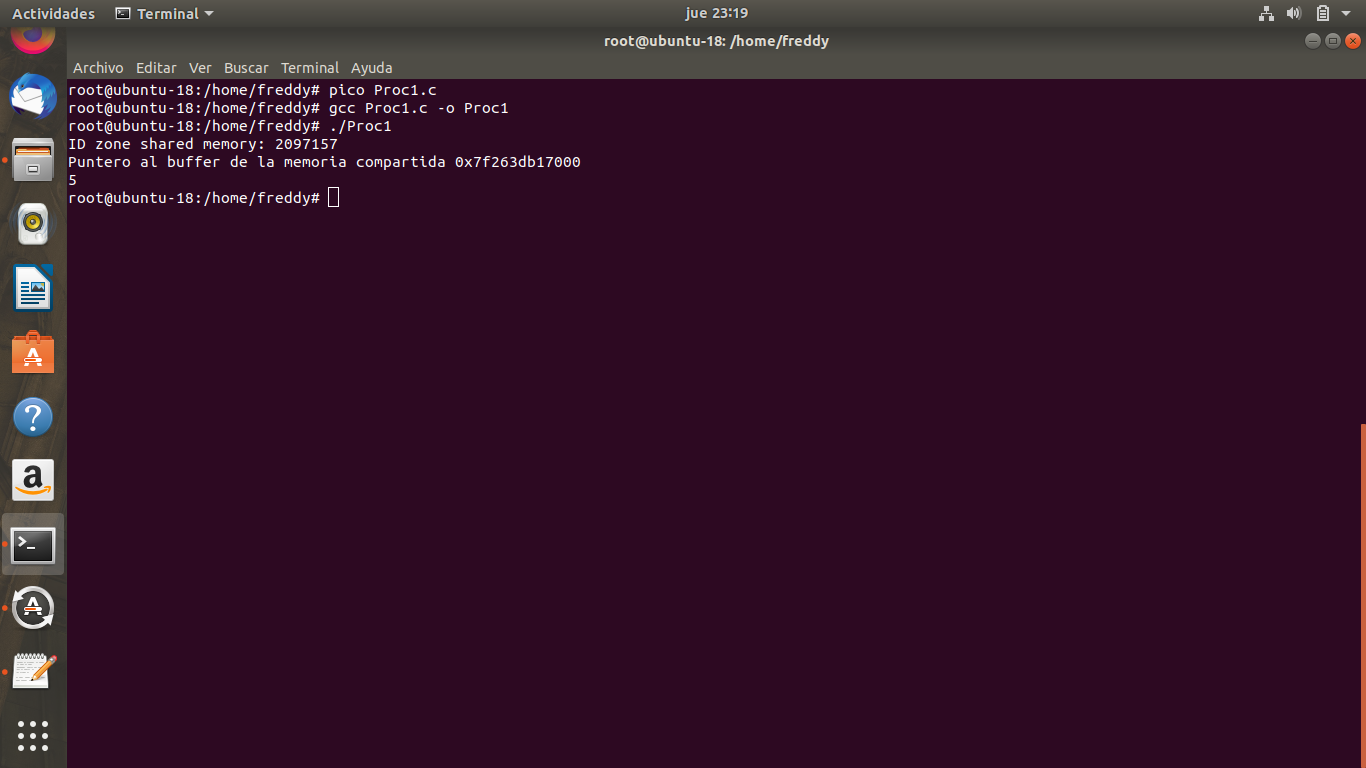
\includegraphics[scale=.35]{proc1.png}
\\
\\
Creando llave para memoria compartida entrando a la zona de memoria, pero crea y declara la memoria compartida,y libera la memoria
\clearpage
\begin{lstlisting}[language=C++, caption={Programa6}]
#include<stdio.h>
#include<unistd.h>
#include<sys/types.h>

int main(){ 
	pid_t pid;
	int n=3,i;
	for(i=0;i<n;i++)
		{
			pid=fork();
			if(pid!=0)
			break;
			else
			pid=fork();
		}
	printf("El padre del proceso %d es %d\n",getpid(),getppid());
}
\end{lstlisting}
\clearpage
Ejecuci\'on\\
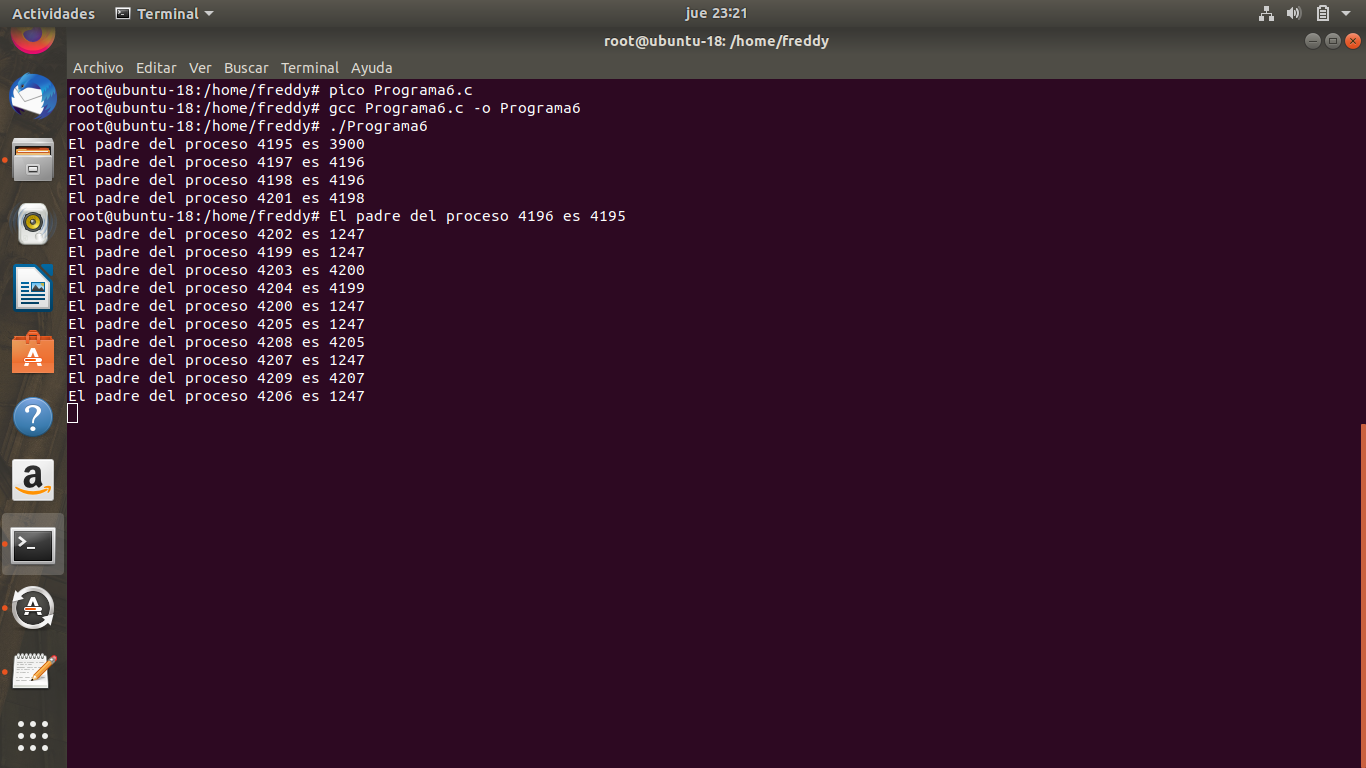
\includegraphics[scale=.35]{programa6.png}
\\
\\
Creando un proceso padre para los demas procesos
\clearpage
\begin{lstlisting}[language=C++, caption={SJF}]
#include <time.h>
#include <stdio.h>
#include <stdlib.h>

void delay(unsigned int mseconds)
{
    clock_t goal = mseconds + clock();
    while (goal > clock());
}


struct proceso
{
	int prioridad;
	char nombre[10];
	int tiempo;
	struct proceso *izq;
	struct proceso *der;
};

int main()
{
	struct proceso *nodo, *p, *q, *nuevo, *cabecera;
	int n, i, prioridad, nombre, tiempo;
	printf("Progrma que crea procesos\n\n");
	
	cabecera =(struct proceso*)malloc(sizeof(struct proceso));
	cabecera->prioridad =0;
	cabecera->nombre[i]=' ';
	cabecera->tiempo= 0;
	cabecera->izq=NULL;
	cabecera->der=NULL;
	
	do
	{
		p=(struct proceso*)malloc(sizeof(struct proceso));
		printf("Deme la prioridad: ");
		scanf("%d", &p->prioridad);
		printf("Nombre del proceso ");
		scanf("%s", &p->nombre);
		printf(" Tiempo: ");
		scanf("%d", &p->tiempo);
		
		if(cabecera->der==NULL)
		{	
			p->der=NULL;
			p->izq=cabecera;
			cabecera->der=p;
		}
		else
		{
			q=cabecera;
			//p->prioridad=prioridad;
			while((((q->der)!=NULL) && ((p->prioridad > (q->der)->prioridad))))
				q=q->der;

			if (q->der==NULL)
			{
				q->der=p;
				p->der=NULL;
				p->izq=q;	
			}			
			else
			{
				p->der=q->der;
				q->der=p;
				p->izq=q;
				p->der->izq=p;
		    }
		}
		printf("agregar otro proceso: [0-NO] [1- SI]:  ");
		scanf("%d", &n);
		printf("\n");
	}while(n!=0);
	
		while(p->der!=NULL)
		p=p->der;
		
		while(p)
		{
		    printf("Nombre %s\n", p->nombre);
			printf("Tiempo %d\n", p->tiempo);
			printf("El prioridad fue %d\n",p->prioridad); 
			for(i=0;i<=p->tiempo;i++)
			{
			printf("Tiempo de ejecucion: %d...\n", i);
			delay(1000);
			}
			p=p->izq;
		}
	}
\end{lstlisting}
\clearpage
Ejecuci\'on\\
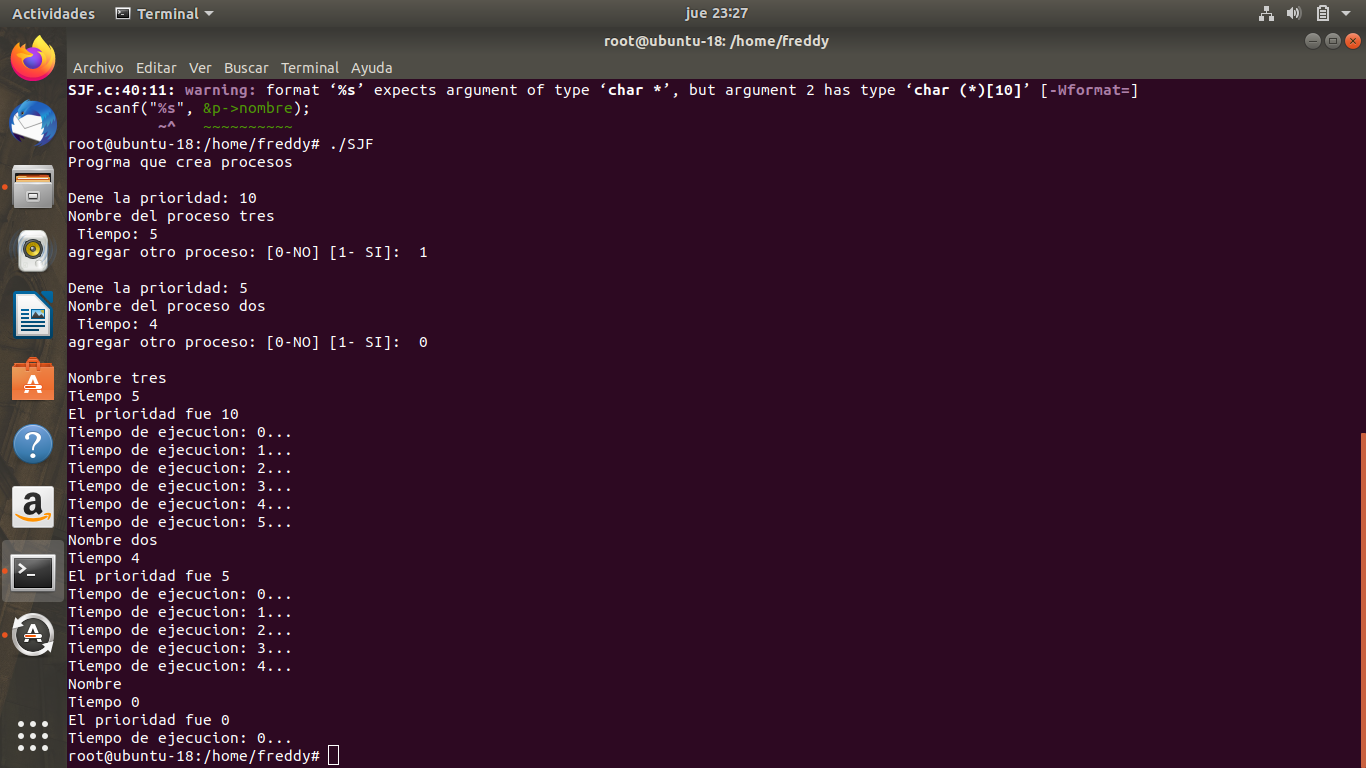
\includegraphics[scale=.35]{sjf.png}
\\
\\
Creando un sincronizador de procesos mediante nodos, lo que realiza es mandar a llamar a los procesos para indicarles su prioridad y el tiempo de cada uno.
\clearpage
\begin{lstlisting}[language=C++, caption={Tubc2}]
#include <fcntl.h>
#include <unistd.h>
#include <stdio.h>
#include <stdlib.h>
#include <string.h>

#define SIZE 512

int main ( char argc, char **argv )
{
  pid_t pid;
  int p[2], readbytes;
  char buffer[SIZE];

  pipe( p );

  if ( (pid=fork()) == 0 )
  { // hijo
    close( p[1] ); /* cerramos el lado de escritura del pipe */

    while( (readbytes=read( p[0], buffer, SIZE )) > 0)
      write( 1, buffer, readbytes );

    close( p[0] );
  }
  else
  { // padre
    close( p[0] ); /* cerramos el lado de lectura del pipe */

    strcpy( buffer, "Esto llega a traves de la tuberia\n" );
    write( p[1], buffer, strlen( buffer ) );

    close( p[1] );
  }
  write( pid, NULL, 0 );
  exit( 0 );
}
\end{lstlisting}
\clearpage
Ejecuci\'on\\
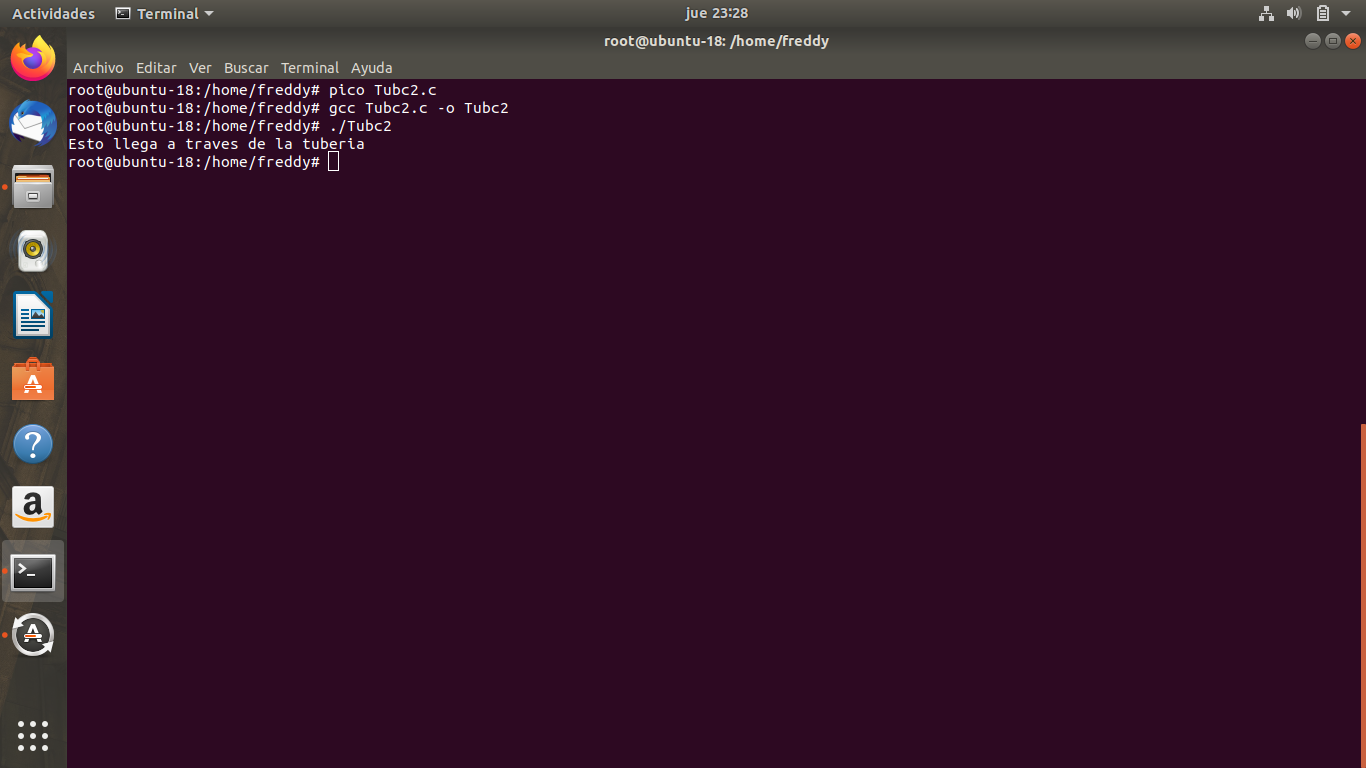
\includegraphics[scale=.35]{tubc2.png}
\\
\\
Creando pipes que llegan mediante tuberias.
\end{document}


